\documentclass[tikz]{standalone}
\usepackage{pgfplots}
\tikzset{
  jumpdot/.style={mark=*,solid},
  excl/.append style={jumpdot,fill=white},
  incl/.append style={jumpdot,fill=black},
}
\usetikzlibrary{arrows.meta,intersections,calc,quotes,angles}
\pgfplotsset{width=7cm,compat=1.18} 
\begin{document}
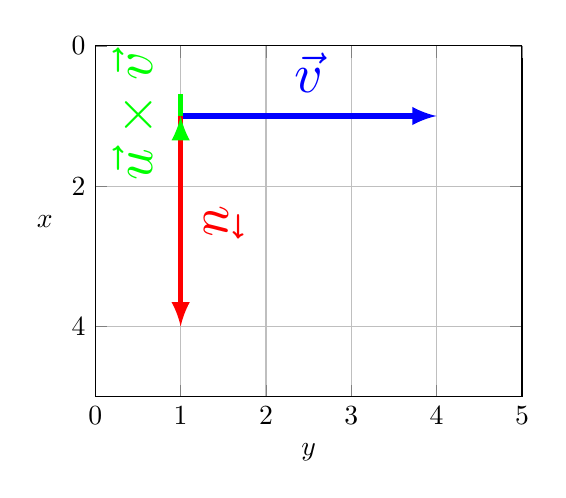
\begin{tikzpicture}
\begin{axis}[
  grid=major,
  xmin=0,
  xmax=5,
  ymin=0,
  ymax=5,
  zmin=0,
  zmax=10,
  xlabel=$x$,
  ylabel=$y$,
  zlabel=$z$,
  view={90}{90},
  %xtick={-3,0,...,5},
  %ytick={-5,0,...,5},
  %ztick={0,3,...,15},
  %xticklabel = \empty,
  %yticklabel = \empty,
  %zticklabel = \empty,
]
\draw[line width=2pt, blue, -latex] (1,1,0) -- (1,4,0) node[sloped,above,midway,scale = 2] {$\vec{v}$};
\draw[line width=2pt, red, -latex] (1,1,0) -- (4,1,0) node[sloped,above,midway,scale = 2] {$\vec{u}$};
\draw[line width=2pt, green, -latex] (1,1,0) -- (1,1,8) node[sloped,above,midway,scale = 2] {$\vec{u} \times \vec{v}$};

%\addplot3 [
%        surf,
%        domain=-10:10,
%        samples=40,
%] gnuplot {10 * sin(x)*sin(y)};
\end{axis};
\end{tikzpicture}
\end{document}